\documentclass[tikz,border=12pt]{standalone}
\usepackage[T1]{fontenc}
\usepackage{mathpazo}
\usepackage{amsmath,amssymb}
\usetikzlibrary{arrows.meta, positioning, calc, fit, decorations.pathreplacing}
\usepackage{pgfplots}
\pgfplotsset{compat=1.18}

\definecolor{stblue}{HTML}{7B97AD}
\definecolor{rwgold}{HTML}{B8995E}
\definecolor{sage}{HTML}{7A9A7E}
\definecolor{dkbrown}{HTML}{3D3530}
\definecolor{wmgray}{HTML}{7B7067}
\definecolor{cream}{HTML}{F9F6F0}
\definecolor{border}{HTML}{D4C9B8}
\definecolor{terracotta}{HTML}{C47A6A}
\definecolor{lavender}{HTML}{907EA0}

\begin{document}
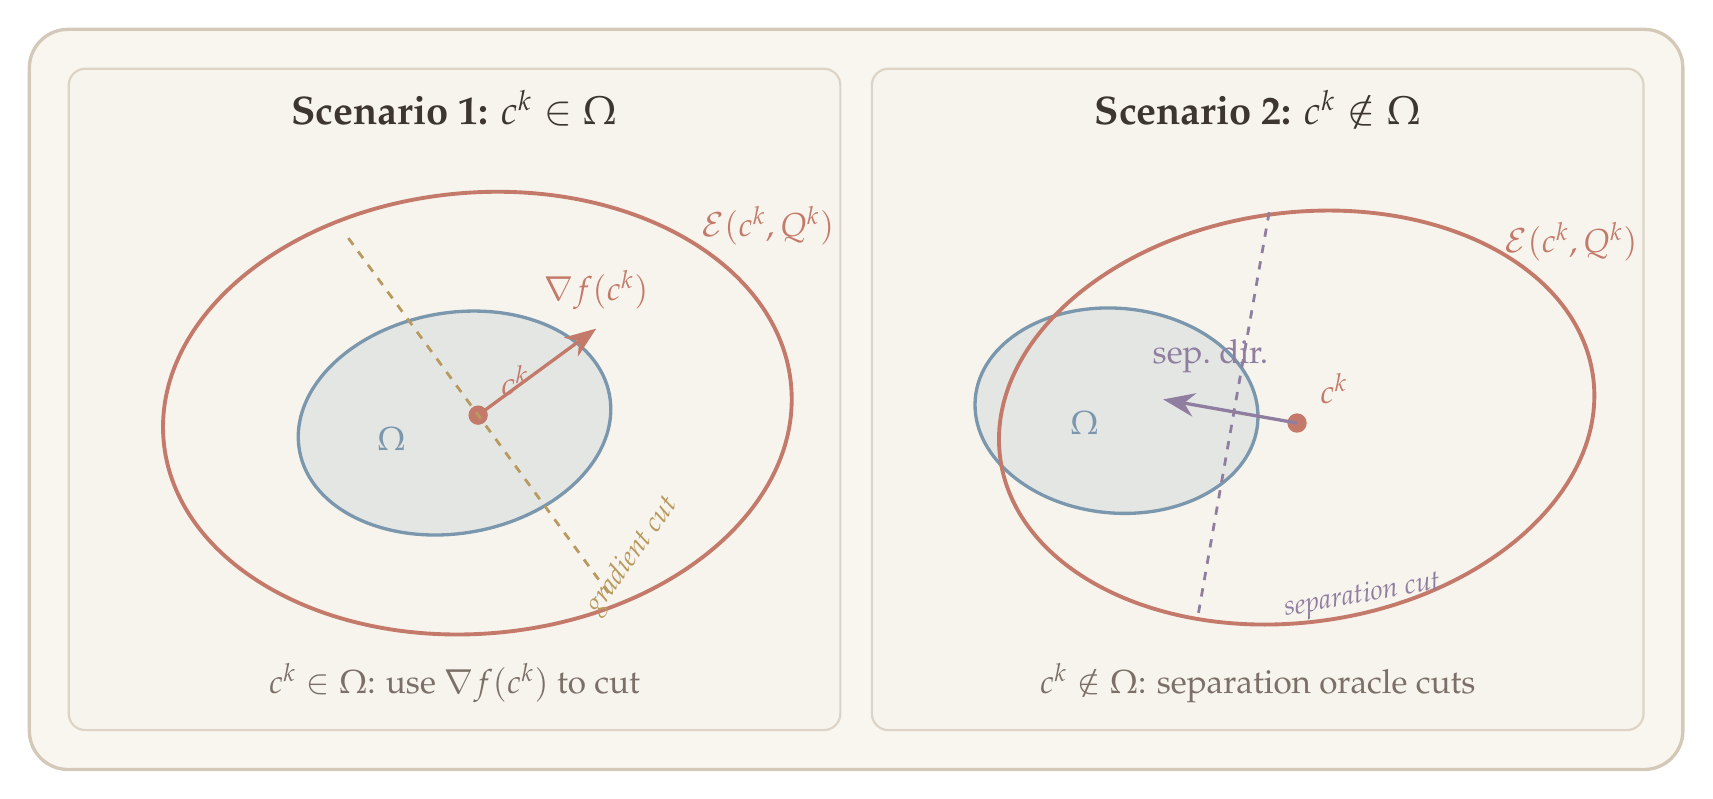
\begin{tikzpicture}[
    >={Stealth[length=4mm, width=3mm]},
    every node/.style={text=dkbrown},
    line width=1.5pt,
  ]

  % Background
  \fill[cream, rounded corners=14pt] (-0.5,-4.2) rectangle (20.5,5.2);
  \draw[border, line width=1.2pt, rounded corners=14pt] (-0.5,-4.2) rectangle (20.5,5.2);

  %%% ============================================================ %%%
  %%% Panel 1: Scenario 1 — c^k in Omega                          %%%
  %%% ============================================================ %%%
  \fill[cream!95!border, rounded corners=6pt] (0.0,-3.7) rectangle (9.8,4.7);
  \draw[border!80, line width=0.8pt, rounded corners=6pt] (0.0,-3.7) rectangle (9.8,4.7);
  \node[font=\Large\bfseries, text=dkbrown] at (4.9,4.2)
    {Scenario 1: $c^k \in \Omega$};

  \begin{scope}[shift={(4.9,0.2)}]
    % Constraint set Omega (stblue filled ellipse)
    \fill[stblue, opacity=0.15, rotate=10] (0,0) ellipse (2.0cm and 1.4cm);
    \draw[stblue, line width=1.2pt, rotate=10] (0,0) ellipse (2.0cm and 1.4cm);
    \node[font=\large\bfseries, text=stblue] at (-0.8,-0.2) {$\Omega$};

    % Ellipsoid E(c^k, Q^k) (terracotta, larger, containing Omega)
    \draw[terracotta, line width=1.4pt, rotate=5]
      (0.3,0.1) ellipse (4.0cm and 2.8cm);
    \node[font=\large\bfseries, text=terracotta, anchor=west] at (3.0,2.5)
      {$\mathcal{E}(c^k, Q^k)$};

    % Center c^k (inside Omega)
    \fill[terracotta] (0.3,0.1) circle (3.5pt);
    \node[font=\large, text=terracotta, anchor=south west] at (0.45,0.2) {$c^k$};

    % Gradient direction arrow (terracotta)
    \draw[terracotta, ->, line width=1.2pt] (0.3,0.1) -- (1.8,1.2);
    \node[font=\large, text=terracotta, anchor=south] at (1.8,1.3) {$\nabla f(c^k)$};

    % Gradient cut line (dashed rwgold, perpendicular to gradient through c^k)
    % Gradient direction: (1.5, 1.1), perpendicular: (-1.1, 1.5)
    \pgfmathsetmacro{\perpx}{-1.1}
    \pgfmathsetmacro{\perpy}{1.5}
    \pgfmathsetmacro{\perplen}{sqrt(\perpx*\perpx+\perpy*\perpy)}
    \draw[rwgold, line width=1.0pt, dashed]
      ({0.3-2.8*\perpx/\perplen},{0.1-2.8*\perpy/\perplen})
      -- ({0.3+2.8*\perpx/\perplen},{0.1+2.8*\perpy/\perplen});
    \node[font=\normalsize\itshape, text=rwgold, anchor=north, rotate=54] at (2.0,-1.5)
      {gradient cut};
  \end{scope}

  % Annotation
  \node[font=\large, text=wmgray, align=center] at (4.9,-3.1)
    {$c^k \in \Omega$: use $\nabla f(c^k)$ to cut};

  %%% ============================================================ %%%
  %%% Panel 2: Scenario 2 — c^k not in Omega                      %%%
  %%% ============================================================ %%%
  \fill[cream!95!border, rounded corners=6pt] (10.2,-3.7) rectangle (20.0,4.7);
  \draw[border!80, line width=0.8pt, rounded corners=6pt] (10.2,-3.7) rectangle (20.0,4.7);
  \node[font=\Large\bfseries, text=dkbrown] at (15.1,4.2)
    {Scenario 2: $c^k \notin \Omega$};

  \begin{scope}[shift={(15.1,0.2)}]
    % Constraint set Omega (stblue filled ellipse, shifted left)
    \fill[stblue, opacity=0.15, rotate=-5] (-1.8,0.0) ellipse (1.8cm and 1.3cm);
    \draw[stblue, line width=1.2pt, rotate=-5] (-1.8,0.0) ellipse (1.8cm and 1.3cm);
    \node[font=\large\bfseries, text=stblue] at (-2.2,0.0) {$\Omega$};

    % Ellipsoid E(c^k, Q^k) (terracotta, larger)
    \draw[terracotta, line width=1.4pt, rotate=8]
      (0.5,0.0) ellipse (3.8cm and 2.6cm);
    \node[font=\large\bfseries, text=terracotta, anchor=west] at (3.0,2.3)
      {$\mathcal{E}(c^k, Q^k)$};

    % Center c^k (outside Omega, to the right)
    \fill[terracotta] (0.5,0.0) circle (3.5pt);
    \node[font=\large, text=terracotta, anchor=south west] at (0.65,0.1) {$c^k$};

    % Separation direction arrow (lavender, pointing from c^k toward Omega)
    \draw[lavender, ->, line width=1.2pt] (0.5,0.0) -- (-1.2,0.3);
    \node[font=\large, text=lavender, anchor=south] at (-0.6,0.5) {sep.\ dir.};

    % Separation cut line (dashed lavender, between c^k and Omega)
    % Perpendicular to separation direction (-1.7, 0.3)
    % Perpendicular direction: (0.3, 1.7)
    \pgfmathsetmacro{\sx}{0.3}
    \pgfmathsetmacro{\sy}{1.7}
    \pgfmathsetmacro{\slen}{sqrt(\sx*\sx+\sy*\sy)}
    % Place the cut line between c^k and Omega, at x ~ -0.3
    \draw[lavender, line width=1.0pt, dashed]
      ({-0.3-2.6*\sx/\slen},{0.15-2.6*\sy/\slen})
      -- ({-0.3+2.6*\sx/\slen},{0.15+2.6*\sy/\slen});
    \node[font=\normalsize\itshape, text=lavender, anchor=west, rotate=10] at (0.2,-2.4)
      {separation cut};
  \end{scope}

  % Annotation
  \node[font=\large, text=wmgray, align=center] at (15.1,-3.1)
    {$c^k \notin \Omega$: separation oracle cuts};

\end{tikzpicture}
\end{document}
